\chapter{A Proactive Approach for Dynamic Load Balancing}
\label{ch:PADLB}
\index{PADLB!Proactive Approach for Load Balancing}
\chaptertoc
\noindent

This chapter discusses our proactive approach for dynamic load balancing. The goal is ``\textit{more information, better load balancing}''. Almost all static load balancing methods assume to have load information or related information to generate a cost model. Thereby, task migration and task distribution rely on prior knowledge to solve balancing. In dynamic load balancing, we do not rely on prior knowledge. Task migration is mainly based on the most current execution status at runtime, such as queue length and execution speed on each process. However, current status information is insufficient, implying that approaches like work stealing or reactive load balancing are seemingly based on speculation. Obviously, speculative balancing operations can be right or wrong for a given period.\\

\section{Overview}
\label{sec:PADLB-Overview}

In our proactive approach, we exploit influence factors related to execution status to predict and provide knowledge of task execution time. The knowledge based on load prediction helps to estimate the level of imbalance. We calculate the number of appropriate tasks and potential processes for task offloading. Benefiting from modern computer architectures and task-based programming models, the approach extends reactive load balancing by employing a dedicated thread for:

\begin{itemize}
	\item Supporting task and system characterization instead of only monitoring queue length.
	\item Using the characterization information to predict load values at runtime. Instead of missing the prior knowledge before running applications, we can generate new knowledge based on predicted load values, e.g., $w$, $L$.
	\item Adapting the prediction knowledge to guide task offloading. We calculate the load difference, the number of tasks, and potential process candidates for better offloading tasks.
\end{itemize}

Our approach is implemented towards a proactive scheme of load balancing, which facilitates different task offloading methods. To be intuitive, Figure \ref{fig:padlb_proact_scheme} shows how this scheme works. The x-coordinate again shows the time progress, while the y-coordinate shows process $P_{i}$ spawning two threads for executing tasks and one dedicated thread for performing load balancing. This thread fits today's modern computing architectures with the increasing number of cores, where one core can be left off to run the dedicated thread (denoted by $T_{comm}$). In practice, our scheme can be deployed through hybrid MPI+OpenMP, which is mostly exploited in various task-based parallel programming models.\\

\begin{figure}[t]
	\centering
	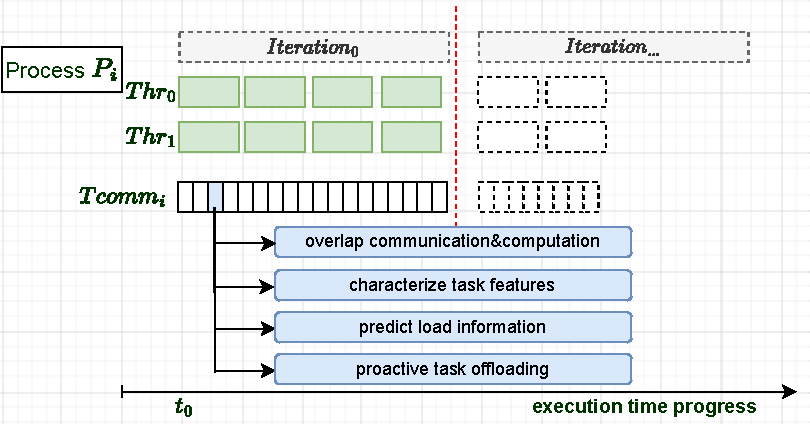
\includegraphics[scale=0.7]{./pictures/padlb_approach/padlb_proact_scheme.pdf}
	\caption{A proactive scheme for task offloading to solve dynamic load balancing in general.}
	\label{fig:padlb_proact_scheme}
\end{figure}

In Figure \ref{fig:padlb_proact_scheme}, we suppose that process $P_{i}$ contains two threads, $Thr_{0}$ and $Thr_{1}$, for executing tasks and one dedicated thread, $Tcomm_{i}$, for communication as well as proactive load balancing. Assuming the execution is iterative, which indicates $Iteration_{0}$, then $Iteration_{1}$, and so on. Different from reactive load balancing, $Tcomm_{i}$ in our approach is driven to perform:

\begin{itemize}
	\item Mainly keeping communication overlapped with computation.
	\item Characterizing task feature and system information along with the corresponding load values, such as $w$, $L$, core frequency, etc.
	\item Training a load prediction model at runtime.
	\item Offloading tasks proactively.
\end{itemize}

%\begin{figure}[t]
%  \centering
%  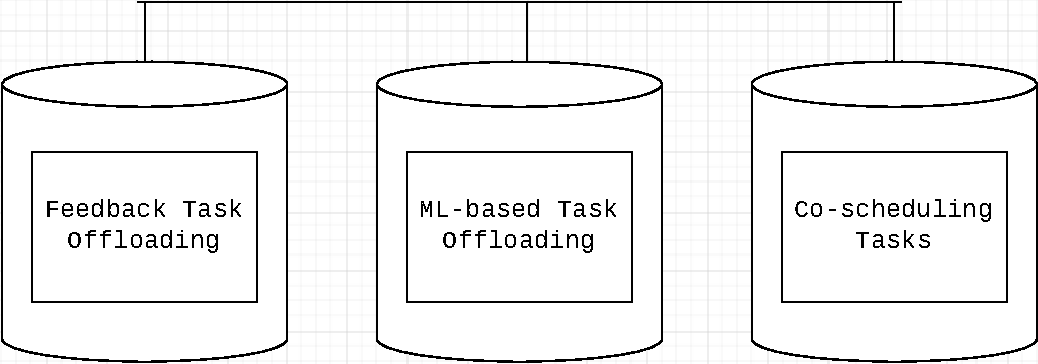
\includegraphics[scale=0.625]{./pictures/padlb_approach/padlb_three_branches_proact_strategies.pdf}
%	\caption{Three branches of task offloading strategies for proactive load balancing approach.}
%	\label{fig:three_branches_proact_strategies}
%\end{figure}

The above operations are what $Tcomm$ can perform separately from the other threads to facilitate load balancing. Furthermore, we can adapt these operations to specific application and system domains. The following sections show different task offloading methods based on our proactive balancing scheme. Specifically, we show two task offloading methods and one extension for co-scheduling tasks across multiple applications, including:

\begin{itemize}
	\item Method 1: feedback task offloading. We introduce method 1 in Section \ref{sec:PADLB-FeedbackLB}.
	\item Method 2: ML-based task offloading, where ``ML-based'' indicates a machine learning based model for online load prediction. Method 2 is described in Section \ref{sec:PADLB-MLbasedTaskOffload}
	\item Extension: co-scheduling tasks across multiple applications. We address this extension in Section \ref{sec:PADLB-CoschedulingTask}.
\end{itemize}

% The load value of each task or each process can be predicted on-the-fly. We use the prediction results to generate an adaptive algorithm for proactive task offloading.

% The extension from proactive load balancing: co-scheduling tasks across multiple applications. ``\textit{Co-scheduling}'' in load balancing also indicates migrating tasks from process to process. However, the scope of co-scheduling tasks here is across multiple applications, and task migration might be between different processes from different applications.

% After an iteration, it will share the information about the prediction, and each process can know the load status before a new iteration starts. Hence, each can plan to balance the load in advance.
 
% Section 4.0 different proactive strategies
%\section{More Information More Balancing Strategies}
\label{sec:PADLB-proactstrategies}
\index{PADLB!Proactive Strategies}

We focus on the perspective of ``\textit{more information more balancing strategies}''. Almost all static load balancing solutions have to assume that they know about load, the number of tasks, or specific information about applications beforehand. After that, the problem can be formulated and solved by optimal algorithms. The optimal solutions also resolve the output: how many tasks are partitioned and which processes/MPI ranks are. We do not have this information ready at runtime for dynamic balancing problems. What we can have is usually queue length status and execution speed. The balancing strategies have to decide which tasks are migrated, from which rank to which rank. We know little about the execution speed based on the number of remaining tasks in queues per rank or even per machine. All in all, the outcome of almost balancing solutions resolves around:
\begin{enumerate}
	\item Which process shares tasks to which process?
	\item And, how many tasks should be migrated at a time?
\end{enumerate}

Differing from work stealing or reactive load balancing, we introduce a new scheme to perform load balancing more proactive. The approach enables task characterization and load prediction at runtime. We then use the prediction to provide the missing knowledge about load at runtime and guide task offloading. Therefore, as mentioned above, we have partial load information to calculate well (1) and (2). Additionally, we can generate different strategies for task offloading.\\

The context in this work is not static or a master-slave scheduling model\footnote{Where, tasks are generated automatically or nested during execution}. Our context is a given distribution of tasks in distributed memory machines. The approach is described as the runtime scheme shown in Figure \ref{fig:padlb_proact_scheme}. We leave one core off to run a dedicated thread along with other execution threads\footnote{Or so-called main threads to execute tasks of the parallel program.}. From the runtime point of view, we can see that our programs are performed with multiple processes or MPI ranks in distributed memory. In which each process spawns multiple threads to execute tasks, and each thread is pinned to one core. Notably, one dedicated thread is pinned to the last core to perform proactive load balancing. For modern computing architectures today, we have many sockets (even GPU as accelerators) in a single machine; a socket has many cores for parallel processing. At the operating system level, one process can spawn as many threads as recommended to fit the maximum number of physical cores per socket. Therefore, this scheme still fits reasonably to modern computing architectures today, even in the future.\\

%While the load balance is expected before running the applications, another challenge could be caused at the system side when some machines/processes can slow down. The unexpected situation needs actions at runtime and faces the challenge of moving tasks around to regain the balance as expected. Suppose there is no prior knowledge to redistribute the tasks. In that case, people have to use work-stealing ideas in principle, and the delay of stealing time on distributed memory is the challenge. Therefore, the approach in this thesis could be described in the inline figure below.\\

\begin{figure}[t]
	\centering
	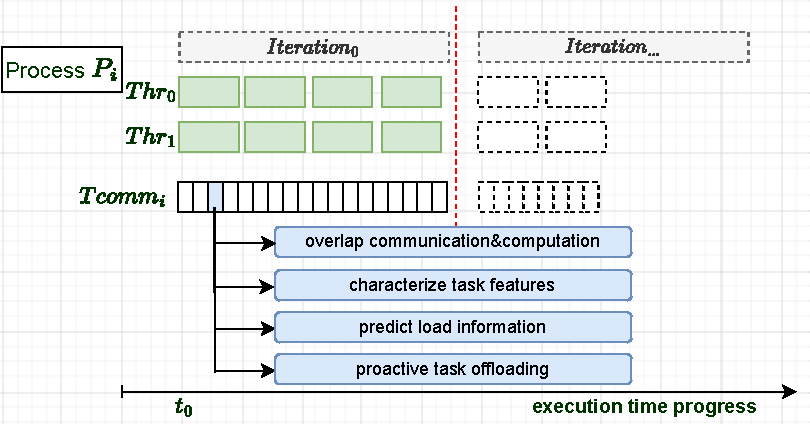
\includegraphics[scale=0.7]{./pictures/padlb_approach/padlb_proact_scheme.pdf}
	\caption{A proactive scheme for task offloading to solve dynamic load balancing in general.}
	\label{fig:padlb_proact_scheme}
\end{figure}

Figure \ref{fig:padlb_proact_scheme} shows our scheme at the level of one process running on one CPU socket. $T0$ and $T1$ illustrate the main execution threads for performing tasks. $Tcomm_{i}$ is the dedicated thread in this process. The x-axis shows the direction of execution time progress. Assume we have iterative execution such as $Iteration_{0}$ - the first execution phase, and so on ( $Iteration_{...}$). Compared to reactive load balancing, our approach extends $Tcomm_{i}$ to have the following properties as shown in Figure \ref{fig:padlb_proact_scheme}:

\begin{itemize}
	\item Because of leaving one core off anyway, $Tcomm$ run asynchronously and plays a role as an assistant for overlapping communication and computation.
	\item $Tcomm$ performs load monitoring, task characterizing, or even system information profiling.
	\item Generating load prediction model on-the-fly.
	\item Provide proactive task offloading to balance the load when necessary.
\end{itemize}

\begin{figure}[t]
  \centering
  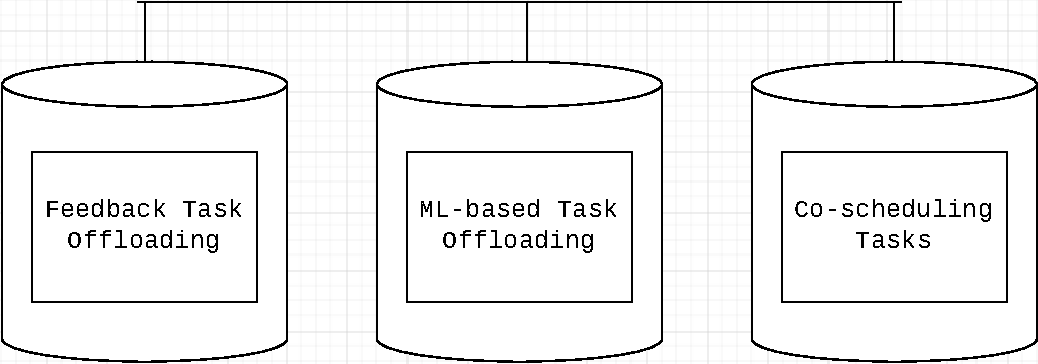
\includegraphics[scale=0.625]{./pictures/padlb_approach/padlb_three_branches_proact_strategies.pdf}
	\caption{Three branches of task offloading strategies for proactive load balancing approach.}
	\label{fig:three_branches_proact_strategies}
\end{figure}

The above properties are what $Tcomm$ can be enabled to do at runtime because it is managed separately from the other threads. Furthermore, we can define it adaptively in application-specific or system-specific domains. This scheme motivates us the idea of one approach toward different task offloading strategies to balance the load. Concretely, we can combine or adjust these properties to make different strategies. We show three strategies in this work as Figure \ref{fig:three_branches_proact_strategies} shows.\\

The first branch is feedback task offloading. The idea behind it is considered as an improved variant of reactive approaches. In terms of iterative applications, the first iteration is still applied reactive balancing operations. Tasks are offloaded from a slow process to a fast one during execution. Unlike the original approach, after the first iteration, we use $Tcomm$ to generate a statistic about local tasks, offloaded tasks, and total load per rank. We can summarize the total load and offloading information over iterations based on the statistic. Following that, a priority function for task offloading is created to tune which process has higher priority for migrating tasks simultaneously. The main purpose is to collect feedback and improve the next iterations. Over time, we can adjust the balancing operations to be more proactive and better in the next iterations. \\

The second branch is ML-based task offloading for load balancing, where ``\textit{ML-based}'' is considered as an online load prediction module. The load value of each task or each process can be predicted on-the-fly, and we use this information to build an adaptive algorithm for balancing. The idea of this branch is to use runtime profiled data to learn runtime values. This is useful in providing knowledge for a balancing strategy. \\

The last branch is co-scheduling tasks for load balancing, where ``\textit{co-scheduling}'' means process-by-process can talk to each other. To be extended, we can think about co-scheduling tasks across multiple applications as an outlook. $Tcomm$ will be the contact person between two or more processes. After an iteration, it will share the information about the prediction, and each process can know the load status before a new iteration starts. Hence, each can plan to balance the load in advance.

%
%\paragraph{Formulation of Influence Parameters}
%\label{PADLB-formulation}
%
%Sed mi sem, commodo et enim a, molestie rutrum nisl. Aliquam sit amet bibendum dui. Nam finibus tempus augue at pretium. Curabitur condimentum magna leo, eu bibendum tellus congue id. Aliquam tempor sed lectus a venenatis. Ut ornare nunc sit amet urna maximus maximus. Nunc tincidunt ex at metus sagittis convallis sit amet ac mi. In luctus nunc sem, a facilisis justo luctus vel. Cras ultricies ex ut quam elementum, sed pharetra ligula tristique. Maecenas fringilla sodales magna quis iaculis. Pellentesque id libero imperdiet, vehicula libero in, fermentum est. Mauris imperdiet risus sit amet hendrerit vestibulum. Curabitur tincidunt enim dui, non auctor leo fringilla vitae. Donec in tellus vitae eros sollicitudin blandit a id neque. Curabitur ante nibh, cursus ut aliquet ultricies, ultricies eget velit. Proin massa ex, scelerisque at tincidunt ac, porta non nibh.


% Section 4.1 feedback load balancing
\section{Feedback Task Offloading}
\label{sec:PADLB-FeedbackLB}
\index{PADLB!Feedback Task Offloading}

The idea behind feedback is an improvement of reactive approach. Applying to iterative applications, the first iteration is kept doing with reactive load balancing. Tasks are offloaded from a slow process to a fast one during execution. After the first iteration, we use $Tcomm$ to generate a statistic on each process about the number of executed tasks in local and remote processes, the total load values of local and remote tasks. The statistic shows how good balancing in the first iteration is. Then, we use this statistic to interpolate the load difference among processes that support an estimation for which processes are overloaded and underloaded. From here, a priority function for task offloading is generated as feedback to drive proactive task offloading in the next iterations.\\

\begin{figure}[t]
	\centering
	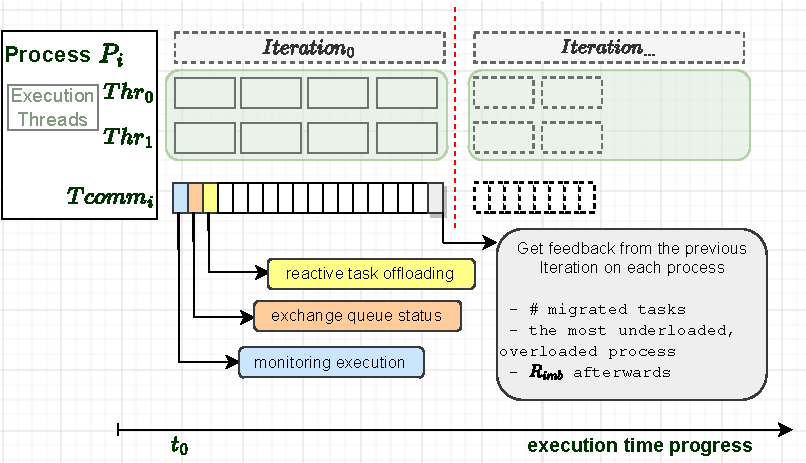
\includegraphics[scale=0.65]{./pictures/padlb_approach/padlb_feedback_lb_idea.pdf}
	\caption{An overview of feedback task offloading through the operations of $Tcomm$.}
	\label{fig:padlb_feedback_task_offloading}
\end{figure}

Figure \ref{fig:padlb_feedback_task_offloading} presents the design of $Tcomm$ to perform feedback task offloading. Again with the coordinates, the x-axis indicates execution time progress. Vertically, we illustrate process $P_{i}$, where its two main threads ($Thr_{0}$, $Thr_{1}$) are shown with executing tasks, $Tcomm_{i}$ with balancing operations. In the first iteration ($Iteration_{0}$), the operations of reactive load balancing are performed the same. For instance, we can see the small rectangles with three different colors. Each rectangle represents an operation in reactive load balancing, where blue is monitoring execution (i.e., queue length), orange is exchanging the status, and yellow is offloading tasks. These operations are repeated until $Iteration_{0}$ is terminated. From here, the arrow at the last rectangle on $Tcomm_{i}$ points to a statistic for feedback.\\

A crucial question is what information is needed for feedback. In this method, we collect the information regarding the efficiency of the first iteration, including:

\begin{itemize}
	\item The number of local and remote tasks executed in a process.
	\item The number of offloaded tasks.
	\item The total load values of local and remote tasks.
	\item The $R_{imb}$ ratio and speed up after reactive load balancing in the first iteration.
\end{itemize}

\begin{algorithm}[t]
\caption{Feedback Task Offloading} \label{alg:feedback_task_offloading}
	\setstretch{1.25}		% for the spacing between lines
	\DontPrintSemicolon % for not showing the semicolon of an empty line command
	\SetNoFillComment		% to align the comment position
	\SetKwInOut{KwIN}{Input}
	\SetKwInOut{KwOUT}{Output}
	\SetKwInOut{KwRET}{Return}
	
	\SetKwFunction{FBba}{feedback\_balancing}
	\SetKwFunction{ASer}{assert}
	\SetKwFunction{EVal}{evaluate}

	% --------------------------------------------
	\; % intended for an empty line as spacing
  % --------------------------------------------
  \KwIN{Array $L^{\text{local}}$\texttt{[]}, $L^{\text{remote}}$\texttt{[]}, $N^{\text{local}}$\texttt{[]}, $N^{\text{remote}}$\texttt{[]}, each has P elements. Where, $L^{\text{local}}\texttt{[i]}$ is local load value; \\
  		$L^{\text{remote}}\texttt{[i]}$ is remote load value; \\
  		$N^{\text{local}}\texttt{[i]}$ is the number of local tasks; and \\
  		$N^{\text{remote}}\texttt{[i]}$ is the number of remote tasks in process $P_{i}$}
  \KwOUT{Array $D_{\text{reference}}\texttt{[]}$: a reference distribution of priorities}
  % --------------------------------------------
	\; % intended for an empty line as spacing
  % --------------------------------------------
  \SetKwProg{Fn}{Procedure}{:}{}
  \Fn{\FBba{\texttt{Array} $L^{\text{local}}$, $L^{\text{remote}}$, $N^{\text{local}}$, $N^{\text{remote}}$}}{
  	\tcc{Check the input}
  	\nl \ASer{$L^{\text{local}}$, $L^{\text{remote}}$, $N^{\text{local}}$, $N^{\text{remote}}$} \\
  	\nl \ASer{$\texttt{flag}_{\text{feedback}}$} \\
		% --------------------------------------------
		\; % intended for an empty line as spacing
		% --------------------------------------------
  	\tcc{Summarize statistic}
		\nl \texttt{Array} $L$ $\leftarrow$ $L^{\text{local}}$ $+$ $L^{\text{remote}}$  \\
		\nl $L_{max}$, $L_{avg}$ $\leftarrow$ maximum and average load based on Array $L$ \\
		\nl $R_{imb}$ $\leftarrow$ calculate imbalance ratio in overall \\
		\nl \EVal{$R_{imb}$} \tcp*[l]{evaluate the efficiency of reactive load balancing in the first/previous iteration}
		% --------------------------------------------
		\; % intended for an empty line as spacing
		% --------------------------------------------
		\tcc{Interpolate the original load values and local tasks based on average}
		\nl \For{$i \leftarrow 0$ \KwTo \texttt{P-1}}{
				\nl $\hat{L}\texttt{[i]}$, $\hat{w}^{\text{local}}\texttt{[i]}$ $\leftarrow$ based on $L^{\text{local}}\texttt{[i]}$, $N^{\text{local}}\texttt{[i]}$ \\
				\nl $\hat{w}^{\text{remote}}\texttt{[i]}$ $\leftarrow$ based on $L^{\text{remote}}\texttt{[i]}$, $N^{\text{remote}}\texttt{[i]}$ \\
		}
		\nl $\hat{L}_{max}$, $\hat{L}_{avg}$ $\leftarrow$ maximum and average load based on \texttt{Array} $\hat{L}$ \\
		\nl $\hat{R}_{imb}$ $\leftarrow$ calculated by $\hat{L}_{max}$, $\hat{L}_{avg}$ \\
		\nl $D_{\text{reference}}$ $\leftarrow$ a reference distribution of priorities if $\hat{R}_{imb}$ $\geq$ $\texttt{Threshold}_{\texttt{imb}}$ \\
		
%		\nl \If{$\hat{R}_{imb} \geq \texttt{Threshold}_{\texttt{imb}}$}{
%				\nl $D_{\text{reference}}[]$ $\leftarrow$ a reference distribution of priorities \\
%		}

		\nl \KwRET{$D_{\text{reference}}$}
  }
  
  % --------------------------------------------
	%\; % intended for an empty line as spacing
  % --------------------------------------------
	%\SetKwProg{Fn}{Procedure}{:}{}
  %\Fn{\FCoo{\texttt{Array} $\texttt{IDLE}^{'}$}}{
  	%\tcc{Check runtime information}
		%\nl $pid$ $\leftarrow$ check process id \\
		%\nl $B$ $\leftarrow$ check average bandwidth information for task migration \\
			
		% --------------------------------------------
		%\; % intended for an empty line as spacing
		% --------------------------------------------
		%\KwRET{$P_{\texttt{victim}}$, $\texttt{num}_{\texttt{offload}}$}
  %}
\end{algorithm}

In case the current iteration is not the first iteration (\texttt{Iteration 0}), feedback requests the iteration called the \textit{previous} iteration. Generally, Algorithm \ref{alg:feedback_task_offloading} shows how the feedback information works on each process. The feedback includes recorded information about the local, remote load, number of local tasks, and number of remote tasks denoted by $L^{\text{local}}$\texttt{[]}, $L^{\text{remote}}$\texttt{[]}, $N^{\text{local}}$\texttt{[]}, $N^{\text{remote}}$ \texttt{[]} respectively. The output is an array of priorities corresponding to each process. The priority gives each a reference number that says offloading tasks (if $> 0$) or receiving tasks (if $< 0$). Their values suggest a reference limit for how many tasks we should offload or receive in a process. These input/output arrays have $P$ elements alluding to the number of involved processes.\\

(1) Procedure \texttt{feedback\_balancing()} checks the input arrays. Then, it is ensured to run only one time every iteration by the flag $\texttt{flag}_{\text{feedback}}$, except for the first iteration of collecting data to give feedback.\\

(2) We summarize a statistic about how good reactive load balancing is performed in the first/previous iteration.\\

The total load value ($L$) per process is calculated by the sum of local and remote load, $L^{\text{local}}$ $+$ $L^{\text{remote}}$. After distributing the values $L$, $L^{\text{local}}$, $L^{\text{remote}}$ around, each process calculates $L_{max}$, $L_{avg}$ that are used to check the imbalance ratio $R_{imb}$. By evaluating $R_{imb}$, we can determine the efficiency of reactive load balancing in the first/previous iteration.\\

(3) The procedure interpolates information about the original load value and task execution time of each process based on average, denoted by $\hat{L}\texttt{[i]}$, $\hat{w}^{\text{local}}\texttt{[i]}$. Also, if the current process executed remote tasks, the corresponding $\hat{w}^{\text{remote}}\texttt{[i]}$ is also estimated. Benefit from $\hat{L}$, we estimate information about $\hat{L}_{max}$, $\hat{L}_{avg}$ $\hat{R}_{imb}$ to check how load difference among processes if reactive load balancing is not applied. Eventually, the difference of $\hat{L}$ and $\hat{L}_{avg}$ associated with $\hat{w}^{\text{local}}\texttt{[i]}$ and $\hat{w}^{\text{remote}}\texttt{[i]}$ supports generating an array of priorities, $D_{\text{reference}}$. As a result, we interpolate the number of tasks that should be offloaded/received to fill the gap between $\hat{L}$ and $\hat{L}_{avg}$. For example, process $P_{i}$ has $D_{\text{reference}}\texttt{[i]} = 99$ that says it should be an offloader, and a reference limit is $99$ tasks.\\

An obvious advantage in feedback task offloading is determining which process is a potential victim for offloading tasks and which is receiving tasks. Another advantage is that we can refer to a limit of how many tasks should be offloaded. These points can drive task offloading in subsequent iterations better.

%In detail, we still rely on the operations of reactive load balancing. However, after each execution phase, we review the progress and use statistics to give feedback for offloading tasks in the next iterations. This can leverage the offloading operations to be more proactive about which processes can potentially be victims. \\

%As we can see in Figure \ref{fig:padlb_feedback_load_balancing}, the first iteration remains reactive task offloading operations. $Tcomm_{i}$ repeatedly monitors each process's queue status, exchanges that information around, and offloads tasks reactively if the imbalance ratio meets. After that, all task offloading data will be recorded for analysis. We make statistics about:




% Section 4.2 ml-based task offloading for LB
\section{ML-based Task Offloading}
\label{sec:PADLB-MLbasedTaskOffload}
\index{PADLB!ML-based Task Offloading}

% ----------------------------------------------------
% Requirement and Design
% ----------------------------------------------------
\subsection{Reprequisite and Design} \label{subsec:ml-based-design}

\begin{figure}[t]
	\centering
	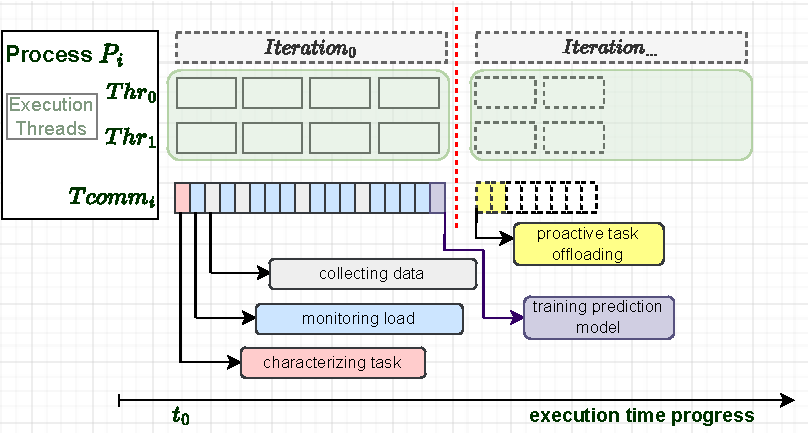
\includegraphics[scale=0.65]{./pictures/padlb_approach/padlb_mlbased_lb_idea.pdf}
	\caption{An overview of ML-based task offloading through the corresponding operations running on $Tcomm$.}
	\label{fig:padlb_mlbased_taskoffload_scheme}
\end{figure}

In feedback task offloading, we use the statistic of executed local/remote tasks after one iteration to give feedback for the next iteration. Task offloading in the upcoming iterations can be performed proactively. When system performance changes significantly or the total load values of processes vary greatly over iterations, this method can be inefficient because the feedback after one iteration might be wrong in the next iteration. In addition, the statistical information after one iteration is finished still lacks coherence with relevant factors on the system side. Therefore, we developed another method using machine learning based on the features of both sides, application and system, for online load prediction.\\

We show that the ML-based idea is feasible because many use cases in HPC are numerical simulations. The program behaviors are iterative execution, where the number of tasks and their arguments are repeated over iterations. The execution phases are also repeated until termination. Therefore, one iteration passed can give useful information for the next iteration. ML-based task offloading method exploits the dedicated thread to combine three main stages:
\begin{itemize}
	\item task characterization
	\item load prediction
	\item proactive task offloading
\end{itemize}

Figure \ref{fig:padlb_mlbased_taskoffload_scheme} shows the design of this method, considered as a reference implementation scheme in practice. For keeping a consistent overview similar to the feedback task offloading method in Figure \ref{fig:padlb_feedback_task_offloading} on Page \pageref{fig:padlb_feedback_task_offloading}, the x-axis shows execution time progress, process $P_{i}$ is illustrated with two threads for executing tasks ($Thr_{0}$, $Thr_{1}$), and $Tcomm_{i}$ is isolated to perform: 

\begin{enumerate}
	\item \texttt{characterizng task}: indicated by red rectangle. We characterize the input arguments of tasks when they are created. Besides that, system information is profiled. We profile CPU core frequency (but not limited to other performance counters that might influence the execution time of tasks, $w$) as a relevant factor on the system side. To define which features are profiled, we can configure them before the application is executed.
	\item \texttt{monitoring load}: indicated by blue rectangle. We record the wallclock execution time ($w$) of each task and the total load ($L$) of each process after an iteration is finished.
	\item \texttt{collecting data}: indicated by grey rectangle. We generate a dataset for training machine learning models based on the characterized and monitored information.
	\item \texttt{training prediction model}: indicated by purple rectangle. After the dataset is generated, $Tcomm$ is triggered to train a prediction model. When the model is successfully trained, it is loaded to predict the load values of tasks/processes for the next iterations.
	\item \texttt{proactive task offloading}: indicated by yellow rectangle. We employ a proactive algorithm for guiding task offloading. Tasks can be offloaded early when the next iterations get started.
\end{enumerate}

Regarding the input and output layers of our prediction model, we formulate their properties as follows.

\begin{itemize}
	\item Prediction Input: In cases of predicting $w$, the input must be the features that we can collect before a task is run, and these features have to reflect the values of task execution time. If the input can only be collected after the termination of tasks, it is irrelevant to apply machine learning at runtime. In cases of predicting $L$, one way can be using the prediction of $w$ values to calculate $L$. Another can use the $L$ values in previous iterations to train and predict $L$ for the next iterations.
	
	\item Prediction Output: is task wallclock execution time ($w$) or total load value of a process after an iteration is done ($L$). $L$ is estimated by the sum of $w$ values of a process. Therefore, $w$ and $L$ can interpolate each other depending on the characteristics of tasks.
\end{itemize}

To be intuitive, Figure \ref{fig:ml_based_workingflow} demonstrates step-by-step the above operations. The demonstration is described with two processes, process $P_{0}$ and process $P_{1}$ following the vertical coordinate. The x-coordinate indicates execution time progress over iterations, such as $Iteration\ 0$, ..., $Iteration\ k$, $Iteration\ k+1$. Assume each process has two threads for executing tasks (so-called two \textit{worker} threads, $Thr_{0}$ and $Thr_{1}$), and the dedicated thread denoted by $Tcomm$. The behavior is an iterative execution, where the number of iterations in a realistic HPC use case might be thousands. This implies a possibility that we can employ ML-based load prediction after a few iterations at the beginning and then apply for proactive task offloading.\\

\begin{figure}[t]
  \centering
  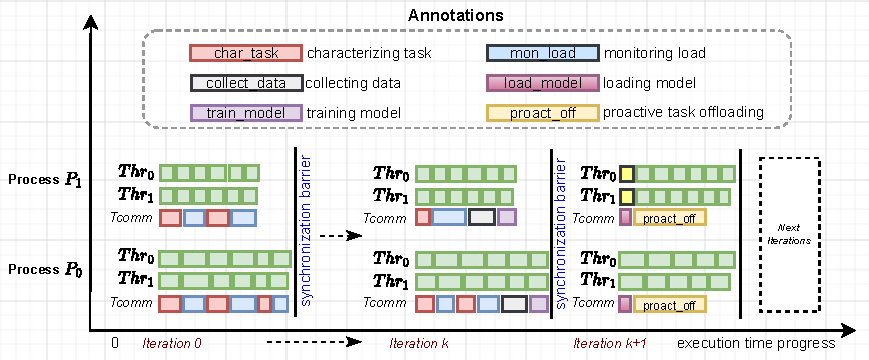
\includegraphics[scale=0.825]{./pictures/padlb_approach/padlb_mlbased_lb_workingflow.pdf}
	\caption{Working flow of ML-based task offloading at runtime.}
	\label{fig:ml_based_workingflow}
\end{figure}

In Figure \ref{fig:ml_based_workingflow}, ``green'' boxes on the rows of threads $Thr_{0}$, $Thr_{1}$ indicate executing local tasks, while ``yellow'' boxes indicate remote tasks. The operations of $Tcomm$ are illustrated by the boxes with different colors, representing different operations when they are performed. Iterations are increasingly indexed by $0$, ..., $k$, $k+1$, and so on. On the rows of $Tcomm$, the operations of characterizing tasks, monitoring load, and collecting data are performed from $Iteration\ 0$ to $Iteration\ k$. These iterations are left for preparing a dataset before training a prediction model. The number of iterations left to generate a dataset might differ depending on user applications. When the dataset is generated, we can see that the operation of training the model is triggered on each process. After training, the model is loaded to predict the load values of the next iterations. Given $Iteration\ k+1$, the model is loaded when it is just getting started. Thereby, we adapt the predicted load results to guide proactive task offloading. Corresponding to the annotation in Figure \ref{fig:ml_based_workingflow}, the boxes with different colors link to the following operations.

\begin{itemize}
	\item \texttt{char\_task} (red): characterizing task. This depends on what we want to characterize. Our case focuses on the input arguments of tasks. Besides, some performance counters, which are enabled to check before a task is executed, can also be involved in \texttt{char\_task}. Therefore, Figure \ref{fig:ml_based_workingflow} shows that \texttt{char\_task} is triggered after tasks are created or before tasks are executed.
	\item \texttt{mon\_load} (blue): monitoring load. We aim at recording the load values ($w$) after tasks are done. This operation can be triggered after executing tasks.
	\item \texttt{collect\_data} (grey): collecting data. This indicates the monitored load values that we use to generate a dataset for training.
	\item \texttt{train\_model} (magenta): training model. When the dataset is generated, \texttt{train\_model} is called. The trained models are mainly regression types to predict load values; however, a custom model is also relevant if we can obtain a good prediction.
	\item \texttt{load\_model} (purple): loading model. This denotes when the model is trained, it is loaded to predict the load values of the next iterations.
	\item \texttt{proact\_off} (orange): proactive task offloading. This annotation indicates that we have prediction results, we can load them to guide proactive task offloading.
\end{itemize}

Concurrently with the other worker threads, $Tcomm$ performs these operations asynchronously. Except when the main execution of worker threads stops, $Tcomm$ is finished. In general, there are some requirements for ML-based task offloading, including:

\begin{itemize}
	\item The operations invoked inside $Tcomm$ should be modularized and callable. Furthermore, they are able to be pre-defined by users. The reason is that online prediction with machine learning cannot be fixed. For different use cases, users might understand their applications better.
	\item Task characterization (\texttt{char\_task}) should be selected with influence features, depending on the application use case. This can affect the overhead of the modules such as \texttt{collect\_data}, \texttt{train\_model}. Compared to prediction problems in other fields, such as computer vision \cite{sebe2006mlincv}, NLP \cite{deng2018dlinnlp}, we have to keep prediction models in load balancing context small and simple due to the scope of available input features.
	\item The ML-based prediction models should be lightweight to avoid overhead in training and loading the models. Regarding accuracy, we do not need a very high result because load balancing is better when relying on the difference in load between different processes.
\end{itemize}

Our use case is iterative, which is especially relevant when applying machine learning to predict execution time over iterations. Furthermore, the input features are not only from the user application side but also from the system side, which can extend to topology information, bandwidth, and memory access pattern. However, to adapt this method to different use cases, we need to answer three questions:
\begin{itemize}
	\item Which input features and how much data are generally relevant?
	\item Which machine learning model is suitable?
	\item Which way can the learning parameters change at runtime?
\end{itemize}

With machine learning, the answer cannot be ``\textit{generalized}'' because prediction and machine learning models cannot be fixed. It should be served on domain-specific applications that we can change and adapt flexibly. The following subsections will clarify our argument through two examples in practice.

% ----------------------------------------------------
% Online Load Prediction Module
% ----------------------------------------------------
\subsection{Online Load Prediction} \label{subsec:online-load-prediction}

The main perspective of ML-based task offloading is that a users' application is considered as a black box. A task is defined by a code region and its data. The code refers to a computation kernel. Users do not need to make an effort to optimize how tasks are executed in parallel. After an execution phase is complete, the programs' flow and task results are given back to the users' control side.\\

During task execution, this is reasonable for predicting load values within a task-based programming model. Particularly, the dedicated thread on each process is suitable to launch a lightweight machine-learning model. Prediction with supervised learning needs input features and output labels to train. To this end, we formulate the input, output, and model using the following parameters:

\begin{itemize}
	\item $IN_{app}$: input features associated with task characterization, e.g., task arguments, data size, code region. We recommend some pre-observation about the task features before choosing which features are influential.
	\item $IN_{sys}$: input features associated with system characterization, i.e., performance counters. We recommend factors that affect execution time, such as core frequency (a min-max range of frequencies), memory access patterns, and cache hit/miss when executing tasks.
	\item $OUT$: output labels. In our context, labels are simplified as the execution time of tasks ($w$) or total load of processes ($L$).
	\item $MODEL$: machine learning algorithms, e.g., linear regression. We use regression algorithms to predict load value because regression is suitable for prediction problems with continuous numerical values. However, other relevant algorithms are also reasonable for specific applications.
\end{itemize}

To illustrate the usage of our online prediction model, we show two examples: matrix multiplication (denoted by \texttt{MxM}) and Sam(oa)$^2$ \cite{Meister2016AMRSamoa}. \texttt{MxM} is a micro-benchmark used to ease the reproducibility of almost all experiments. In \texttt{MxM}, a task is defined by a \texttt{MxM} compute kernel. The input arguments include matrix \texttt{A}, \texttt{B}, and matrix \texttt{C} is the output argument. Sam(oa)$^2$ is an adaptive mesh refinement framework used for oceanic HPC applications/simulations. The design of this framework is based on the numerical analysis of space-filling curves.\\

%\noindent \textbf{A. \texttt{MxM} as an example}\\
\subsubsection{Example: \texttt{MxM} matrix multiplication}
\label{subsubsec:mxm-online-prediction}

On the side of users, the input arguments of a task are matrices, and their sizes can impact the task execution time ($w$). Therefore, we configure the model inputs as matrix size, core frequency, and the model output as task execution time. The matrix size can be collected right after a task is created, and core frequency can also be quickly checked from the system call of operating system. Assuming that each process holds a number of $T_{i}$ tasks ($i$ denotes process $P_{i}$) and we have $P$ processes in total; then, a dataset for training online load prediction can be formatted as the following.

{\small
\begin{align*}
&\textbf{Input}	&	&	&	&	&\textbf{Output} \\
   ---&---		&                ---&----				&									&		&------	\\
	&IN_{app}   &                &IN_{sys}      &                 &   &OUT    \\
   ---&---		&                ---&----				&									&		&------	\\
m_{0} &= 256	&		\text{feq}_{0}	&= 1185.6		&		\rightarrow		&		&w_{0}	\\
m_{1} &= 128	&		\text{feq}_{1}	&=  800.1		&		\rightarrow		&		&w_{1}	\\
m_{2}	&= 512	&		\text{feq}_{2}	&=  900.9		&		\rightarrow		&		&w_{2}	\\
m_{4}	&= 100	&		\text{feq}_{4}	&= 1800.0		&		\rightarrow		&		&w_{4}	\\
m_{3}	&= 256	&		\text{feq}_{3}	&= 1361.8		&		\rightarrow		&		&w_{3}	\\
\cdot\cdot\cdot & & \cdot\cdot\cdot & & & &  \cdot\cdot\cdot 
\end{align*}
}%

With $IN_{app}$, $m_{j}$ represents a matrix size corresponding to a task (task $j$) in a process. The notation $j$ in this case means that suppose process $P_{i}$ has a number of $T_{i}$ tasks, then task $j$ belongs to $T_{i}$ ($j$ simply points to a task index or ID). The value of $m_{j}$ can be normalized as the number of elements or the volume in memory. Here, we use the number of elements, such as $256$ for a matrix of $256 \times 256$ elements. Similarly, with $IN_{sys}$, $\text{feq}_{j}$ represents the core frequency checked before a task is scheduled to execution, where $j$ also points to a corresponding task. The value of $\text{feq}_{j}$ is roughly available to characterize before executing a task. We cannot make sure $100\%$ that $\text{feq}_{j}$ can accurately reflect a task's load value. However, this system feature can relate to the runtime before and after a task is executed. Additionally, $\text{feq}_{j}$ can represent how we combine application and system features to predict the load. In a process, we might have many tasks that explain the input layer indexed by $0$, $1$, $2$, etc. With $OUT$, we show a corresponding execution time of a task, namely $w_{0}$, $w_{1}$, etc.\\

%\noindent \textbf{B. Sam(oa)$^2$ as an example}\\
\subsubsection{Example: Sam(oa)$^2$}
\label{subsubsec:samoa-online-prediction}

Sam(oa)$^2$ is an adaptive mesh refinement framework developed for oceanic HPC applications. The use cases of Sam(oa)$^2$ include tsunami, earthquake, or environmental simulations. Therefore, we use Sam(oa)$^2$ as a real iterative application for experiments in our work. In Sam(oa)$^2$, this framework utilizes a concept of grid sections where each section is processed by a single thread \cite{Meister2016AMRSamoa}. A traversed section is an independent computation unit, which is defined as a task. Following the canonical approach of cutting the grid into parts of uniform load, tasks per process are uniform. A set of tasks belonging to different processes might not correspond to the same load. Sam(oa)$^2$ supports hybrid MPI+OpenMP programming models. Hence, we can port its application into a task-based parallel application, where each process assigned tasks refers to MPI ranks\footnote{``Rank'' and ``process'' are used interchangeably in the following sections.}. An MPI rank supports multiple OpenMP threads to execute tasks.\\

By characterizing Sam(oa)$^2$, we observe that predicting the $w$ value of each task in a process is not very useful to estimate load imbalance. The tasks are uniform, and their $w$ values (wallclock execution time) are alike in the same iteration. Notably, the total load values ($L$) per process are changed over iterations, and $L$ can be predicted based on a chain of $L$ values in the previous iterations. This example shows how we can adjust the influence features to predict the load values depending on application characterization.\\

For input data layer, we use the total load value of an iteration ($L^{I}_{i}$), where $L^{I}_{i}$ denotes the load of process $P_{i}$ in iteration $I$. The dimension of input features depends on how many complete iterations we want to specify. For instance, if we take $4$ complete iterations and assume the current iteration as a prediction target is $I$, then the array of input features includes $L^{I-4}_{i}$, $L^{I-3}_{i}$, $L^{I-2}_{i}$, $L^{I-1}_{i}$, where $L^{I}_{i}$ is the prediction output. To trace back the $w$ values of each task from the predicted $L^{I}_{i}$, the estimation can be based on the average of $w$ through $L$ and the number of assigned tasks per process because tasks are known with uniform load following the characterization of Sam(oa)$^2$.\\

The following samples show a layout of the dataset with two processes, process $P_{0}$ and process $P_{1}$. We keep the $L$ values of $4$ complete iterations to generate a sample dataset.

{\small
\begin{align*}
\textbf{Dataset on } &\textbf{process $P_{0}$} \\
   ---&---	      	\\
&\textbf{Input}	& &	&	& & & & &	&\textbf{Output} \\
   ---&---  & & & &	& & & & &------	\\
	&IN_{app} & & & & & & & & &OUT    \\
   ---&---  & &	& & & & & & &------	\\
L^{0}_{0} &=0.029  &  L^{1}_{0} &=0.062  &  L^{2}_{0} &=0.040  &  L^{3}_{0} &=0.070	& \rightarrow &	 &L^{4}_{0} =0.035  \\
L^{1}_{0} &=0.062  &  L^{2}_{0} &=0.035  &  L^{3}_{0} &=0.070  &  L^{4}_{0} &=0.035	& \rightarrow &	 &L^{5}_{0} =0.062  \\
L^{2}_{0} &=0.035  &  L^{3}_{0} &=0.070  &  L^{4}_{0} &=0.035  &  L^{5}_{0} &=0.062	& \rightarrow &	 &L^{6}_{0} =0.035  \\
L^{3}_{0} &=0.070  &  L^{4}_{0} &=0.035  &  L^{5}_{0} &=0.062  &  L^{6}_{0} &=0.035	& \rightarrow &	 &L^{7}_{0} =0.070  \\
L^{4}_{0} &=0.035  &  L^{5}_{0} &=0.062  &  L^{6}_{0} &=0.035  &  L^{7}_{0} &=0.070	& \rightarrow &	 &L^{8}_{0} =0.035  \\
L^{5}_{0} &=0.062  &  L^{6}_{0} &=0.035  &  L^{7}_{0} &=0.070  &  L^{8}_{0} &=0.035	& \rightarrow &	 &L^{9}_{0} =0.062  \\
\cdot\cdot\cdot & & \cdot\cdot\cdot & & \cdot\cdot\cdot & & \cdot\cdot\cdot & & & & \cdot\cdot\cdot              
\end{align*}
}%

{\small
\begin{align*}
\textbf{Dataset on } &\textbf{process $P_{1}$} \\
   ---&---	      	\\
&\textbf{Input}	& &	&	& & & & &	&\textbf{Output} \\
   ---&---  & & & &	& & & & &------	\\
	&IN_{app} & & & & & & & & &OUT    \\
   ---&---  & &	& & & & & & &------	\\
L^{0}_{1} &=0.030  &  L^{1}_{1} &=0.072  &  L^{2}_{1} &=0.036  &  L^{3}_{1} &=0.062	& \rightarrow &	 &L^{4}_{1} =0.036  \\
L^{1}_{1} &=0.072  &  L^{2}_{1} &=0.036  &  L^{3}_{1} &=0.062  &  L^{4}_{1} &=0.036	& \rightarrow &	 &L^{5}_{1} =0.061  \\
L^{2}_{1} &=0.036  &  L^{3}_{1} &=0.062  &  L^{4}_{1} &=0.036  &  L^{5}_{1} &=0.061	& \rightarrow &	 &L^{6}_{1} =0.036  \\
L^{3}_{1} &=0.062  &  L^{4}_{1} &=0.036  &  L^{5}_{1} &=0.061  &  L^{6}_{1} &=0.036	& \rightarrow &	 &L^{7}_{1} =0.070  \\
L^{4}_{1} &=0.036  &  L^{5}_{1} &=0.061  &  L^{6}_{1} &=0.036  &  L^{7}_{1} &=0.070	& \rightarrow &	 &L^{8}_{1} =0.035  \\
L^{5}_{1} &=0.061  &  L^{6}_{1} &=0.036  &  L^{7}_{1} &=0.070  &  L^{8}_{1} &=0.035	& \rightarrow &	 &L^{9}_{1} =0.064  \\
\cdot\cdot\cdot & & \cdot\cdot\cdot & & \cdot\cdot\cdot & & \cdot\cdot\cdot & & & & \cdot\cdot\cdot 
\end{align*}
}%

In process $P_{0}$, the dataset is normalized until iteration $9$. We do not need to use the profiled features from the system side in this example, such as core frequency, because the total load value in an iteration can be predicted based on the previous iterations. We exploit four previous iterations; therefore, there are four parameters in the input layer, i.e., the $L$ values of iteration $0$, $1$, $2$, $3$. These are denoted by $L_{0}$, $L_{1}$, $L_{2}$, $L_{3}$, representing $IN_{app}$. The output layer, $OUT$, points to the $L$ value of iteration $4$ shown as the first row in the dataset. Similarly, proceeding further until iteration $9$, we have a dataset including $6$ rows of input and output features. Likewise, we have the same dataset layout with process $P_{1}$.\\

After training, each process has its own prediction model. Before the next iterations begin, these models are loaded in advance at $Tcomm$ and predict the total load values.\\

To guide proactive task offloading, prediction results on each process need to be exchanged. After that, each can adapt these predicted values to a proactive task offloading algorithm introduced in the next subsection.\\

\begin{table}[b]
\caption{The input-output features for training a load prediction model in \texttt{MxM} and Sam(oa)$^2$.}
\centering
\scalebox{0.9}{
\begin{tabular}{|m{0.7cm}|m{1.5cm}|m{2.2cm}|m{2.2cm}|m{2.2cm}|m{2.2cm}|}
\hline
\textbf{No.} & \textbf{App.}  & \textbf{Task} & \textbf{$IN_{app}$} & \textbf{$IN_{sys}$} & \textbf{$OUT$} \\ \hline
\textbf{1}   & \texttt{MxM} & \texttt{MxM} kernel & matrix sizes & core freq (Hz) & load/task ($w$) \\ \hline
\textbf{2}   & Sam(oa)$^2$ & grid traversal & previous $L_{i}$ & $\emptyset$ & next $L_{i}$ \\ \hline
\end{tabular}}
\vspace{-1.0em}
\label{tab:dataset_mxm_samoa}
\end{table}

For an overview, we summarize the input and output parameters of both examples, \texttt{MxM} and Sam(oa)$^2$ in Table \ref{tab:dataset_mxm_samoa}. The overview emphasizes that our load prediction model relies on the influence features we can obtain to configure prediction models. Therefore, different applications might need different configurations before running.\\

\begin{figure}[t]
  \centering
  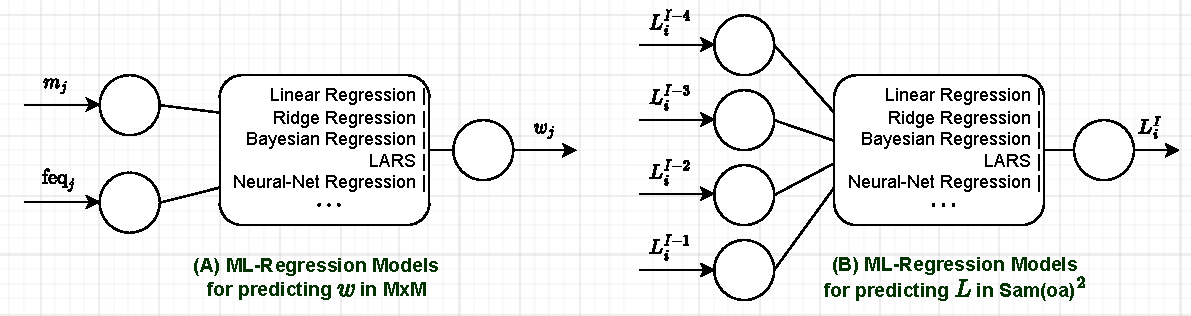
\includegraphics[scale=0.7]{./pictures/padlb_approach/padlb_ml_algorithms.pdf}
	\caption{Machine learning regression models and algorithms that can be applied in \texttt{MxM} and Sam(oa)$^2$.}
	\label{fig:ml_reg_algorithms}
\end{figure}

Regarding what is prepared to train an online prediction model, Figure \ref{fig:ml_reg_algorithms} shows the flow from input to output. In the middle, we highlight possible machine learning models ($MODEL$) that can be applied to predict the target. These are machine learning regression algorithms \cite{james2013introml}, e.g., Linear, Ridge, Bayesian, LARS regression, etc. Figure \ref{fig:ml_reg_algorithms} (A) shows the models for \texttt{MxM}, and (B) for Sam(oa)$^2$. \\

Technically, these algorithms are lightweight to implement. With the requirements of load prediction at runtime, they are simple to customize. Besides that, the main point of load prediction for balancing problems is not how a predicted value of $L$ or $w$ is highly accurate, while we mainly focus on how the imbalance between processes along with an acceptable accuracy.

% ----------------------------------------------------
% ML-based Proactive Task Offloading Algorithms
% ----------------------------------------------------
\subsection{Proactive Task Offloading Algorithm} \label{subsec:proact-offload-algorithm}

After loading the prediction, the prediction output is transferred to the algorithm, which is used to guide task offloading. We call it ``proactive task offloading'' algorithm. The prediction results are simplified for the algorithm's input. In general, the input and output include:

\begin{itemize}
	\item \texttt{Input}: includes array \texttt{L} and array \texttt{N}. Array \texttt{L} is the predicted load values of processes, which can be specified as $[$ $L_{0}$, $...$, $L_{P-1}$ $]$. Array \texttt{N} is the number of assigned tasks on each process, depending on a distribution of tasks before execution. The length of array \texttt{L} and \texttt{N} is the number of involved processes, $P$. Each process has array \texttt{L} after it exchanges the predicted load value ($L_{i}$) with the others. Following that, we can calculate imbalance ratio ($R_{imb}$).
	
	\item \texttt{Output}: is the reference number of how many tasks should be offloaded on each process. Obviously, if a process is underloaded, its reference number of offloaded tasks is zero. If this reference number is $> 0$, the corresponding process should offload tasks proactively.
\end{itemize}

% In addition, we can extract the load of each task ($w$) directly or indirectly based on the prediction model. Suppose $w$ is a prediction target, $w$ is obviously available and can infer $L$. Otherwise, if $L$ is a prediction target, $w$ can be estimated on an average with a given number of tasks.

\begin{algorithm}[t]
\caption{Proactive Task Offloading} \label{alg:proact_offload}
	\setstretch{1.25} % for the spacing between lines
	\DontPrintSemicolon % for not showing the semicolon of an empty line command
	\SetNoFillComment % to align the comment position
  \SetKwFunction{ABS}{ABS}
  \SetKwFunction{ASSERT}{ASSERT}
  % \SetKw{Break}{break}
  % \SetKw{Off}{OFF}
  \SetKwInOut{KwIN}{Input}
  \SetKwInOut{KwOUT}{Output}
	% --------------------------------------------
	\; % intended for an empty line as spacing
  % --------------------------------------------
  \KwIN{Array \texttt{L}, \texttt{N}, where each element \texttt{L[i]}, \texttt{N[i]} indicates the predicted load value and the number of assigned tasks on process \texttt{$P_{i}$}.}
  \KwOUT{Table \texttt{TB} is a 2D array, which can be represented as a matrix. The size of \texttt{TB} is \texttt{P}$\times$\texttt{P}. Each element indicates the number of tasks that a process should offload.}
  % --------------------------------------------
	\; % intended for an empty line as spacing
  % --------------------------------------------
  \nl New Array $\hat{\texttt{L}} \leftarrow$ Sort \texttt{L} by the load values \\
  
  \nl $\texttt{L}_{avg}$ $\leftarrow \sum_{i=0}^{\texttt{P}-1}\frac{\texttt{L}[i]}{\texttt{P}}$ \tcp*[l]{Estimate the average load value}
  
  \nl New Array \texttt{R}; \texttt{TB} \tcp*[l]{\texttt{R} has \texttt{P} elements denoting the total load of remote tasks per rank, \texttt{TB} has \texttt{P}$\times$\texttt{P} elements as mentioned} % \scriptsize for smaller font

  \nl \For{$i \leftarrow 0$ \KwTo \texttt{P-1}}{
  		\nl \If{$\hat{\texttt{L}}[i] < \texttt{L}_{avg}$}{
      		\nl $\Delta_{under} \leftarrow \texttt{L}_{avg} - \hat{\texttt{L}}[i]$ \tcp*[l]{Calculate the load value under average}
					\nl \For{$j \leftarrow \texttt{P-1}$ \KwTo $0$}{
							\nl \If{$\hat{\texttt{L}}[j] > \texttt{L}_{avg}$}{
									\nl $\Delta_{over} \leftarrow \hat{\texttt{L}}[j] - \texttt{L}_{avg}$ \tcp*[l]{Calculate the load value over average}
									\nl $\hat{w} \leftarrow$ Estimate the load per task and \ASSERT($\Delta_{over} \geq \hat{w}$)\\
									\nl \eIf{$\Delta_{over} \geq \Delta_{under}$}{
										\nl $\texttt{N}_{\texttt{off}}, \texttt{L}_{\texttt{off}} \leftarrow$ Estimate the number of tasks to offload and the amount of load for these remote tasks by $\hat{w}, \Delta_{under}$ \\
									  }{
										\nl $\texttt{N}_{\texttt{off}}, \texttt{L}_{\texttt{off}} \leftarrow$ Estimate the number of tasks to offload and the amount of load for these remote tasks by $\hat{w}, \Delta_{over}$ \\
									}
									\nl \texttt{Update} $\Delta_{under}$, $\hat{\texttt{L}}$ at the index $i$ and $j$ based on $\texttt{N}_{\texttt{off}}$, $\texttt{L}_{\texttt{off}}$ \\
									\nl \texttt{Update} $\texttt{N}[j]$, $\texttt{R}[j]$; \texttt{TB} at the index $(i,j)$, $(j,i)$, $(j,j)$ \\
									\nl \texttt{Break} if \ABS($\Delta_{under}, \texttt{L}_{avg}$) $< \hat{w}$
							}
					}
  		}
  }
  \nl \KwRet{\texttt{TB}}   
\end{algorithm}

Algorithm \ref{alg:proact_offload} shows the proactive task offloading algorithm. As mentioned above, array \texttt{L} and array \texttt{N} contain the predicted load values of processes\footnote{``Process'' and ``rank'' might be used interchangeably to describe the text in Algorithm \ref{alg:proact_offload}} and the given number of assigned tasks per process. The length of each array is \texttt{P}, where \texttt{P} is the number of involved processes. For the output, this algorithm generates a result named \texttt{TB}, which can be addressed as a 2D array (a table, or a matrix) to record the following values.
\begin{itemize}
	\item The number of remaining tasks in original processes.
	\item The number of offloaded tasks from the original process to others.
	\item The indices of each element in \texttt{TB} indicate which process should offload tasks to which process.
\end{itemize}

Step-by-step, we create a new array $\hat{\texttt{L}}$ at Line $1$ to store the sorted load values of array \texttt{L}, and calculate the average load value ($\texttt{L}_{avg}$) based on $\sum_{i=0}^{\texttt{P}-1}\frac{\texttt{L}[i]}{\texttt{P}}$ at Line $2$. The average is considered an optimal balanced value. To track the amount of load that receives from the offloaded tasks, Algorithm \ref{alg:proact_offload} allocates array \texttt{R}. We call this amount of load remote load values, and each element of array \texttt{R} is the remote load value of a corresponding process.\\

To track the number of tasks, array \texttt{TB} records the number of local tasks (remaining tasks in an original process) and remote tasks (offloaded tasks to other processes if yes). We use \texttt{TB} as a tracking or recording table that we can technically implement it as a matrix. The size of \texttt{TB} is \texttt{P}$\times$\texttt{P}. However, we just need the upper or lower triangle part, where its diagonal represents the number of local tasks, and the others indicate the number of offloaded tasks. For example, if the value of \texttt{TB[i,j]} $> 0$ ($i \neq j$), process $P_{i}$ should offload a number of \texttt{TB[i,j]} tasks to process $P_{j}$.\\

In detail, Algorithm \ref{alg:proact_offload} is described by two main loops. The outer loop processes each victim. Note that ``victim'' here indicates the process which receives offloaded tasks from the others, while ``offloader'' indicates the process which migrates tasks. Compared to the average load value, a victim is underloaded ($\hat{\texttt{L}}[i] < \texttt{L}_{avg}$), while an offloader is overloaded ($\hat{\texttt{L}}[i] > \texttt{L}_{avg}$). Typically, the underloaded value between process $P_{i}$ and $\texttt{L}_{avg}$ is calculated at Line $6$, named $\Delta_{under}$. This implies that process $P_{i}$ needs to be filled with a load of $\Delta_{under}$ to balance the load. The inner loop goes backward for each offloader. The overloaded load ($\Delta_{over}$) between process $P_{j}$ and $\texttt{L}_{avg}$ is then calculated at Line $9$.\\

To compute the number of tasks for offloading, we need to know the load value $w$ of each task. With an online load prediction model, if our prediction target is the load $w$, then the value $w$ of each task is obviously available. Otherwise, if our prediction target is the total load $L$ of each process, then the value $w$ can be estimated as an average between $L$ and the given number of assigned tasks per process. Therefore, we call $\hat{w}$ an estimated load value of each task (Line $10$ in Algorithm \ref{alg:proact_offload}). This depends on application characteristics to estimate $w$ and also depends on user configuration before execution.\\

Afterward, the number of offloaded tasks ($\texttt{N}_{\texttt{off}}$) and the total offloaded load ($\texttt{L}_{\texttt{off}}$) are calculated. We cannot fix the calculation of $\texttt{N}_{\texttt{off}}$. Instead, our algorithm shows that $\texttt{N}_{\texttt{off}}$ offers several possibilities to calculate. This should be tuned in a proper way because we know load information at runtime relying on the load prediction model. Basically, we can divide $\Delta_{under}$ by the task execution time, $w$, to estimate $\texttt{N}_{\texttt{off}}$, and simultaneously multiply it with a coefficiency. The coefficiency implies that there are some scenarios that we have to consider for tuning the calculation of $\texttt{N}_{\texttt{off}}$ and $\texttt{L}_{\texttt{off}}$. For example:
\begin{itemize}
	\item Scenario 1: the imbalance is caused by performance slowdown in some processes, where the number of assigned tasks on each process is the same, while the load values $w$ of tasks differ, depending on where the tasks are executed. Following that, the values of $\texttt{N}_{\texttt{off}}$ and $\texttt{L}_{\texttt{off}}$ after calculation need to be adjusted, e.g., $2\%$, $5\%$, or $7\%$ more because the tasks on the original process moving to the remote process can be performed faster.

	\item Scenario 2: the execution speed of all processes is stable. The difference in task distribution causes imbalance. Then, the value of $\texttt{N}_{\texttt{off}}$ can be calculated by $\Delta_{under}$ and the predicted value $w$.
\end{itemize}

In further steps of the algorithm, the values of $\Delta_{under}$, $\hat{\texttt{L}}$, \texttt{N}, \texttt{R}, \texttt{TB} will be updated at the corresponding indices. At line $16$, the absolute values between $\Delta_{under}$ and $\texttt{L}_{avg}$ are compared with $\hat{w}$ to check whether or not the current offloader has enough tasks to fill up a load of $\Delta_{under}$. If not, we will go for another candidate (another offloader). In terms of complexity, if we have \texttt{P} processes in total, where \texttt{Q} is the number of victims, \texttt{P-Q} will be the number of offloaders; then the algorithm takes $O$\texttt{(Q(P-Q))} steps. Our implementation is published and described in detail on a GitHub repository, referring to this link at footnote\footnote{\label{notechamtool}https://github.com/chameleon-hpc/chameleon-apps/tree/master/tools/tool\_load\_prediction}.

%\noindent \textbf{A. An example with \texttt{MxM}} \\
\subsubsection{Example: \texttt{MxM} matrix multiplication}
\label{subsubsec:mxm-applied-proactlb}

\noindent To demonstrate the algorithm, we use the example of the \texttt{MxM} matrix multiplication again. For reproducibility purposes, we artificially generate the imbalance of \texttt{MxM} by distributing different numbers of tasks on different processes. The execution speed of all processes is kept stable, and all tasks have uniform load (similar load). The level of imbalance here can be easily varied by the number of tasks per process, intending to create a specific imbalance scenario. Particularly, we assume having $8$ MPI processes. The example in this sub-section is shown with an imbalance ratio of $\approx 4.0$. We distribute the number of tasks on each rank before execution, such as $T_{0}=800$, $T_{1}=100$, $T_{2}=50$, $T_{3}=50$, $T_{4}=50$, $T_{5}=50$, $T_{6}=90$, $T_{7}=90$. A task is defined by a compute kernel of \texttt{MxM}, and the program execution is set iteratively by $5$ iterations in total. The first iteration is left to predict the load values. In the following steps, we assume that the prediction results per process are already obtained and available to input the algorithm.\\

\begin{figure}[t]
  \centering
  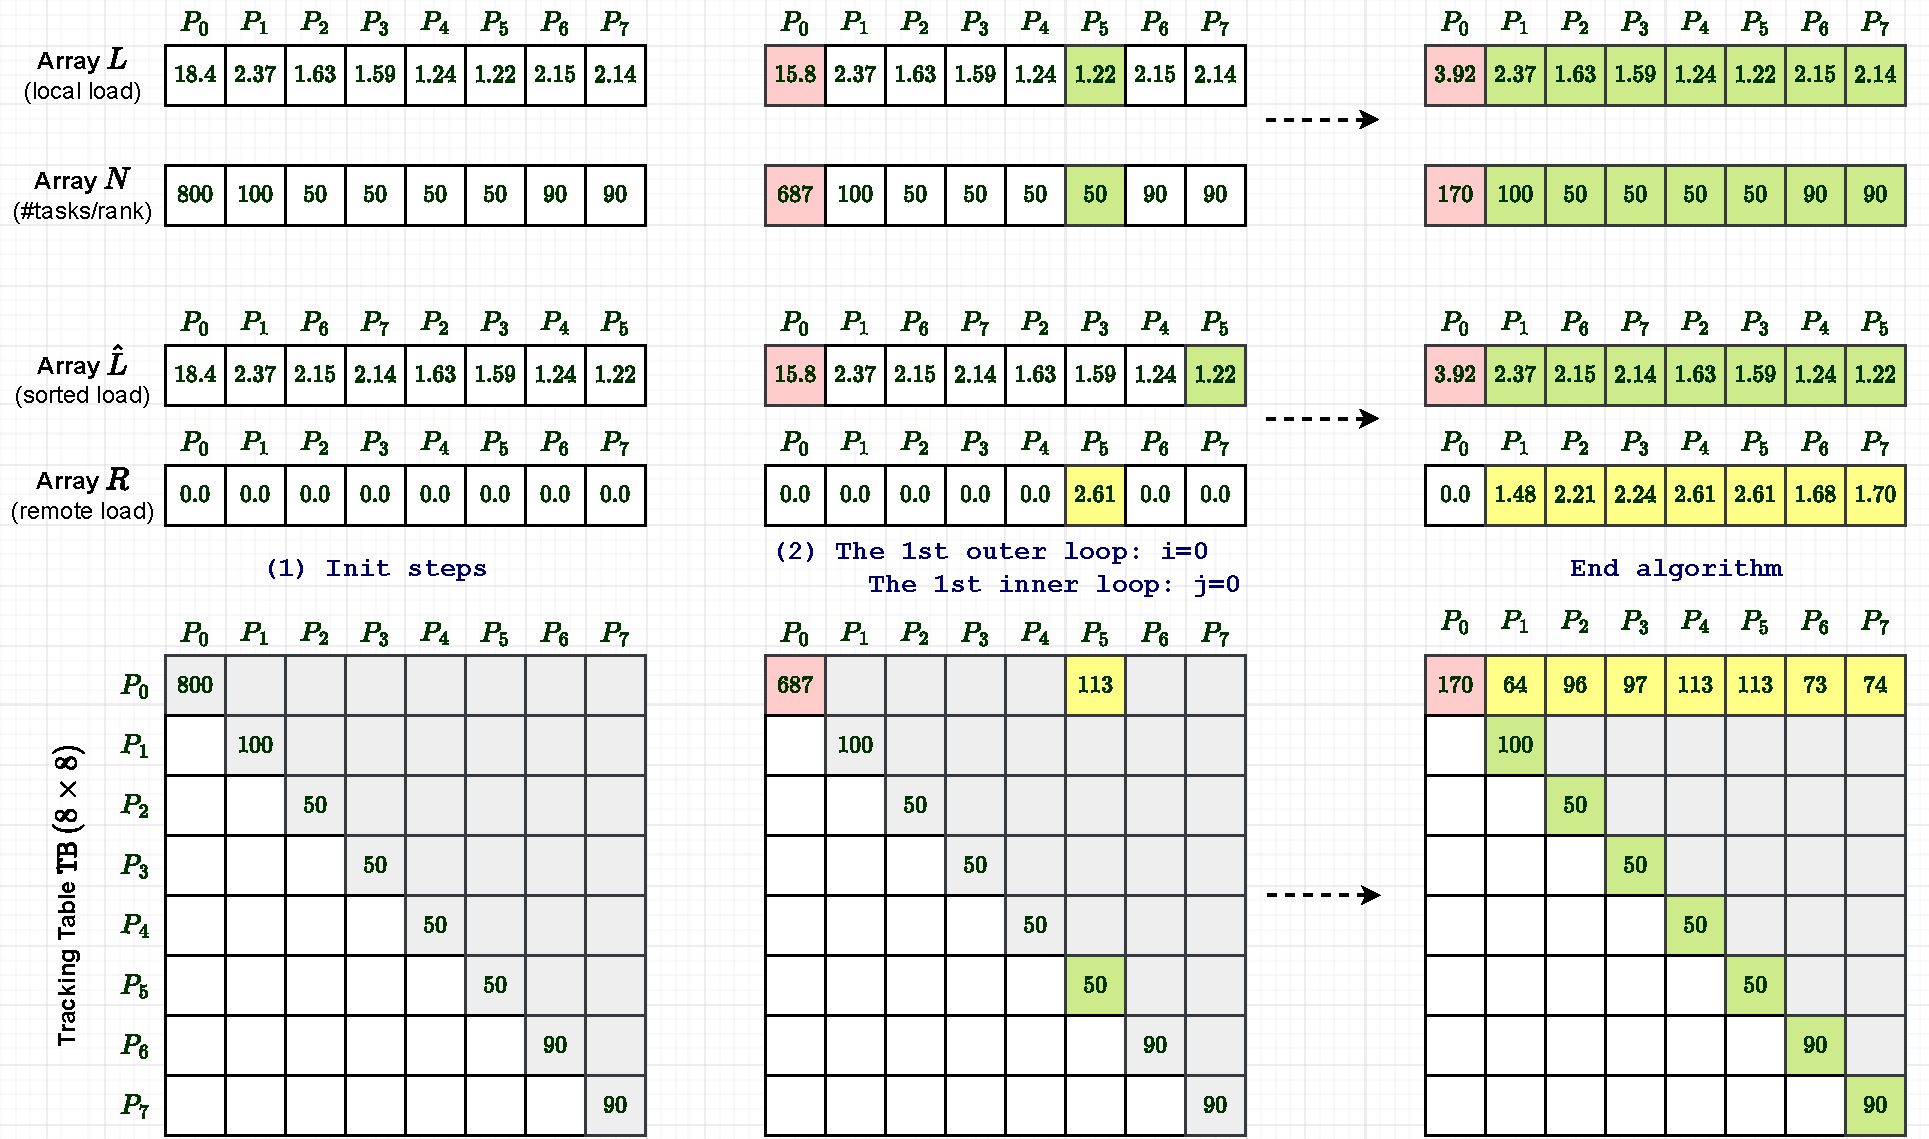
\includegraphics[scale=0.475]{./pictures/padlb_approach/padlb_proact_taskoffload_mxm_example.pdf}
	\caption{An example of applying the proactive task offloading algorithm on \texttt{MxM} matrix multiplication.}
	\label{fig:example_proact_offload_mxm}
\end{figure}

Figure \ref{fig:example_proact_offload_mxm} illustrates the initialization step (denoted by \texttt{(1)}), first loop (denoted by \texttt{(2)}) and last loop (denoted by \texttt{End algorithm}) of Algorithm \ref{alg:proact_offload} to visualize how we can calculate the recommended number of tasks for offloading. From left to right are three columns of the illustrated arrays, each representing a working step.\\

The initialization step \texttt{(1)} is shown in the first column. From here, the input is shown with array \texttt{L} and array \texttt{N}. Array \texttt{L} contains the local load values of each process, which are predicted and exchanged from the prediction module. Array \texttt{N} contains the given numbers of assigned tasks on each process. Here, process $P_{0}$ is the most overloaded process with a total execution time of $18.4$, and process $P_{1}$ occupies the second position. Corresponding to the number of assigned tasks, process $P_{0}$ has the largest number of tasks ($800$), and its load stands the biggest value. In the first stage, array \texttt{L} is sorted by the load values and named $\hat{\texttt{L}}$. With $\hat{\texttt{L}}$, we create another array \texttt{R} to keep tracking the remote load when tasks are migrated around from one process to another. Their local load values will be changed alongside their remote load values. Table \texttt{TB} tracks the number of local and remote tasks, where the diagonal line accounts for the local tasks. The upper triangle part of \texttt{TB} (cells are shaded grey) accounts for the number of remote tasks that should be offloaded. This example shows one of the extreme imbalance cases, where we have one overloaded process, and it has to migrate tasks to other processes for balancing.\\

In the second step \texttt{(2)}, the outer loop of Algorithm \ref{alg:proact_offload} is processed. We traverse the first victim, process $P_{5}$. At this time, the $P_{5}$'s predicted load is $1.22$. Compared to the average load ($\approx 3.84$), process $P_{5}$ needs around a load of $2.62$ to be balanced. Then, we go to the inner loop, traversing the first offloader, which has the load value $L$ $>$ $\texttt{L}_{avg}$. Obviously, process $P_{0}$ is an appropriate offloader, so we can calculate how much overloaded it holds compared to the average load. At this time, we estimate that process $P_{0}$ has enough tasks to offload to process $P_{5}$, and a load of $\approx 2.62$ is equivalent to $113$ tasks from process $P_{0}$. Afterward, the arrays such as \texttt{L}, \texttt{N}, \texttt{R}, and \texttt{TB} are updated. As Figure \ref{fig:example_proact_offload_mxm} shows, \texttt{TB} is updated at the indices $[0,0]$, $[5,5]$, and $[0,5]$, where the element $\texttt{TB}[0,5]$ highlights the number of tasks that we should offload from process $P_{0}$ to $P_{5}$.\\

Ultimately, in the last step (\texttt{End algorithm}), we see a fully updated \texttt{TB}. This case has only process $P_{0}$ changing local tasks and local load, while the others only receive remote tasks. The results suggest offloading tasks earlier at the beginning of the upcoming iteration. For instance, process $P_{0}$ should offload $64$ tasks to $P_{1}$, $96$ to $P_{2}$, and so on. The ML-based task offloading method shows that we can proactively offload tasks early with a guided plan. When we have prediction results, Algorithm \ref{alg:proact_offload} is applied the same step-by-step. Therefore, we do not need to show another example of how this algorithm works for Sam(oa)$^2$.

%\noindent \textbf{B. Task Migration Strategies} \\
\subsubsection{Task Migration Strategies}
\label{subsubsec:migration-strategies}

Following the output of Algorithm \ref{alg:proact_offload}, we can refer to how many tasks should be offloaded as well as migrated from which process to which potential victim proactively. While ``reactive'' is based on the most current status to react immediately to migrating tasks, we can anticipate a relative plan for migrating tasks with respect to ``proactive''. Based on the result of the example shown in Figure \ref{fig:example_proact_offload_mxm}, we know that process $P_{0}$ should offload $64$ tasks to process $P_{1}$, $96$ to process $P_{2}$ at the beginning when a new iteration starts executing tasks. Following this point, the questions are: Which process should migrate the tasks first? And how should we migrate the tasks according to a reference number such as $64$, $96$? Therefore, with the ML-based task offloading method, we can also define a better task migration strategy.\\

\begin{figure}[t]
  \centering
  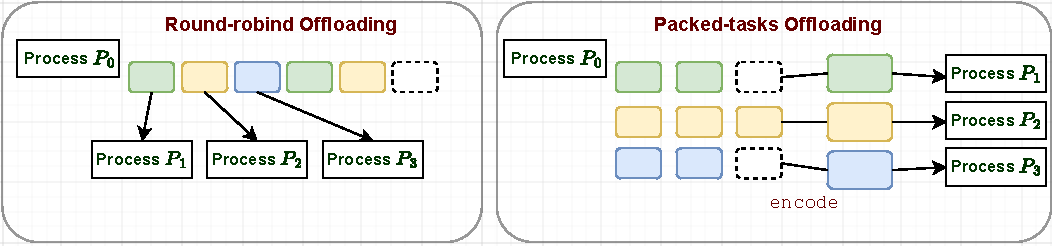
\includegraphics[scale=0.7]{./pictures/padlb_approach/padlb_migration_strategies.pdf}
	\caption{Two related strategies for task migration.}
	\label{fig:two_migration_strategies}
\end{figure}

In Figure \ref{fig:two_migration_strategies}, we propose two task migration strategies in the context of ML-based task offloading. These two migration strategies can be useful if one process sends tasks to multiple victims. Specifically, we call them:
\begin{itemize}
	\item round-robin task offloading
	\item packed-tasks offloading
\end{itemize}

Round-robin sends task by task; for example, we know that process $P_{0}$ needs to offload $64$ tasks to process $P_{1}$, $96$ tasks to process $P_{2}$, etc. Then, the round-robin strategy will take the $1^{st}$ task to $P_{1}$, the $2^{nd}$ task to $P_{2}$, and repeat the progress until all tasks are sent.\\

In contrast, packed-tasks offloading encodes all $64$ tasks, which are planned to be sent to process $P_{1}$, as a package and sends the package at once. After that, we continue to encode $96$ tasks, send the whole package to process $P_{2}$ at once, and so on.

% To be extended, we can think about applying topology information of HPC systems to drive task migration better.


% Section 4.3 coscheduling task for LB
\section{Extension: Co-scheduling Tasks across Multiple Applications}
\label{sec:PADLB-CoschedulingTask}
\index{PADLB!Co-scheduling Tasks for Load Balancing}

\begin{algorithm}[t]
\caption{Proactive Co-scheduling Tasks} \label{alg:proact_coschedule_task}
	\setstretch{1.25}		% for the spacing between lines
	\DontPrintSemicolon % for not showing the semicolon of an empty line command
	\SetNoFillComment		% to align the comment position
	\SetKwInOut{KwIN}{Input}
	\SetKwInOut{KwOUT}{Output}
	\SetKwInOut{KwRET}{Return}
	
	\SetKwFunction{FEst}{estimate\_IDLE}
	\SetKwFunction{FCoo}{proact\_coordinate\_TASK}
	\SetKwFunction{ASer}{assert}
	\SetKwFunction{CHec}{check}
	\SetKwFunction{DSis}{distribute}
	\SetKwFunction{REcv}{receive}
	\SetKwFunction{SEnd}{send}
	\SetKwFunction{OFfl}{offload}
	% --------------------------------------------
	\; % intended for an empty line as spacing
  % --------------------------------------------
  \KwIN{Array of involved processes, P elements in range [$P_{10}$, $P_{11}$, ..., $P_{ij}$], where $i$ indicates application index, $j$ is the process index in that corresponding application.}
  \KwOUT{$\texttt{IDLE}^{'}$: Array of sorted idle time corresponding to the process indices; \\
  				$P_{\texttt{victim}}$: Process victims for offloading tasks; \\
  				$\texttt{num}_{\texttt{offload}}$: The number of tasks for offloading at a point in time.}
  % --------------------------------------------
	\; % intended for an empty line as spacing
  % --------------------------------------------
  \SetKwProg{Fn}{Procedure}{:}{}
  \Fn{\FEst{\texttt{Array} $P[]$}}{
  	\tcc{Get load prediction}
  	\nl $pid$ $\leftarrow$ check process id \\
  	\nl $L_{pid}^{'}$ $\leftarrow$ get load prediction \\
		% --------------------------------------------
		% \; % intended for an empty line as spacing
		% --------------------------------------------
  	\tcc{Exchange load prediction}
		\nl Array $L^{'}$ $\leftarrow$ get predicted load values of other processes \\
		\nl $L^{'}_{max}$ $\leftarrow$ maximum load \\
		\nl Array $\texttt{IDLE}$ $\leftarrow$ estimating idle slots based on $L^{'}_{max}$ \\
		\nl $\texttt{IDLE}^{'}$ $\leftarrow$ sorting the array $\texttt{IDLE}$ \\
		% --------------------------------------------
		% \; % intended for an empty line as spacing
		% --------------------------------------------
		\KwRET{$\texttt{IDLE}^{'}$}
  }
  
  % --------------------------------------------
	\; % intended for an empty line as spacing
  % --------------------------------------------
	\SetKwProg{Fn}{Procedure}{:}{}
  \Fn{\FCoo{\texttt{Array} $\texttt{IDLE}^{'}$}}{
  	\tcc{Check runtime information}
		\nl $pid$ $\leftarrow$ check process id \\
		\nl $B$ $\leftarrow$ check average bandwidth information for task migration \\
		
		\tcc{At the side of idle processes}
		\nl \eIf{\CHec{$\texttt{idle}$}}
		{
			\nl \DSis{$\texttt{IDLE}_{pid}$, $B_{pid}$, $Q_{pid}$} \tcp*[l]{share idle info around}
		
		}{
		\tcc{At the side of busy processes}
			\nl \If{\REcv{$\texttt{idle}$}}{
					\nl Assign $pid_{\texttt{idle}}$, $pid_{\texttt{busy}}$ \\
					\nl \ASer{$\texttt{diff}_{Q_{pid}}$ $>$ $\alpha$} \tcp*[l]{$\alpha$ is a constant limiting the minimum number of remaining tasks that we can make co-scheduling with other processes}
					\nl $\texttt{max}_{\texttt{offload}}$ $\leftarrow$ $\frac{\texttt{IDLE}_{pid_{idle}} \times \bar{B}}{\texttt{data\_size}/task}$ \\
					\nl $\texttt{num}_{\texttt{offload}}$ $\leftarrow$ $\frac{\texttt{IDLE}_{pid_{\texttt{idle}}}}{w^{'}_{pid_{\texttt{busy}}}}$ \\
					\nl \ASer{$\texttt{num}_{\texttt{offload}}$ $<$ $\texttt{max}_{\texttt{offload}}$ and $Q_{pid_{\texttt{busy}}}$} \\
					\nl \SEnd{$\texttt{request}[\texttt{num}_{\texttt{offload}}$, $Q_{pid_{\texttt{busy}}}]$} \\
			}
			
			\nl \If{\REcv{$\texttt{confirm}$}}{ \tcp*[l]{offload tasks afterward if we receive an acceptance}
					\nl \OFfl{$\texttt{num}_{\texttt{offload}}$}
			}
		}				
		% --------------------------------------------
		% \; % intended for an empty line as spacing
		% --------------------------------------------
		\KwRET{$P_{\texttt{victim}}$, $\texttt{num}_{\texttt{offload}}$}
  }
\end{algorithm}

This section introduces an extension based on our proactive load balancing approach, ``co-scheduling tasks across multiple applications,'' which is considered a method for balancing the load not only within an application but multiple applications. $Tcomm$ is still dedicated to handling task migration, but the scope is extended to multiple applications running simultaneously. The principle is mainly migrating tasks from one process to another, but we perform on different applications. Therefore, this method refers to be called ``co-scheduling'' tasks.\\

$Tcomm$ plays the role of a communication channel, where one process in a program\footnote{A program implies that an application is launched at runtime.} can share information with another process running in another program. Following that, the imbalance in a single application can now share the load not only among its processes, but also the other involved applications. There are three main stages:

\begin{enumerate}
	\item Task characterization and load prediction: $Tcomm$ is also deployed to characterize tasks and predict their load values. This stage provides a knowledge to estimate how many tasks we can migrate.
	
	\item Idle slot selection: We can detect idle slots in the application based on task characteristics and load prediction. This phase helps estimate how long a task will take and how much idle time can be suitable for task migration.
	
	\item Prediction exchange and task migration: $Tcomm$ exchanges the prediction information between processes among different applications. If there is an acceptance for sharing tasks, we migrate several tasks from a busy process of the current program to a process with idle slots of the other program.
\end{enumerate}

To enable these stages for co-scheduling tasks, (1) tasks need to be migratable among processes on both sides of involved applications. This implies that different applications need to be enabled for sending or receiving tasks in terms of configuration in advance. If one application meets idle slots, it is feasible to migrate tasks across applications. (2) Our method might not be relevant for task-based applications that feature dynamic task creation because we do not know how many tasks are created before execution.\\

We describe the method and its steps in Algorithm \ref{alg:proact_coschedule_task}. The input is an array of process indices of involved applications [$P_{10}$, $P_{11}$, ..., $P_{ij}$], where $i$ indicates the index of application, $j$ indicates the index of process belonging to that application. The expected outputs include an idle-time array of processes sorted by the idle values ($\texttt{IDLE}^{'}$), process victims ($P_{\texttt{victim}}$) for migrating tasks, and the estimated number of tasks for migrating at once ($\texttt{num}_{\texttt{offload}}$). We clarify the method with two procedures in Algorithm \ref{alg:proact_coschedule_task}:
\begin{itemize}
	\item \texttt{estimate\_IDLE()}
	\item \texttt{proact\_coordinate\_TASK()}
\end{itemize}

First, the procedure \texttt{estimate\_IDLE()} indicates the stage of online load prediction and idle-time estimation. We assume the prediction result is already available at this function. The data collection techniques and training models are similar to the procedure mentioned in Section \ref{sec:PADLB-MLbasedTaskOffload}. $Tcomm$ is triggered to train a prediction model asynchronously while other threads are executing tasks. From here, we just need to load the trained model. Therefore, the procedure shows the predicted load values of the current process ($pid$) at Line $2$. Afterward, we share this value with other processes in the original and other applications to estimate idle time. This mainly intends for different types of tasks. For example, we distinguish computation tasks and communication/IO tasks, where communication/IO tasks are just waiting for communication procedures. Then, we can fill the waiting gaps with tasks from other processes or from other applications. Following the exchange of predicted values, each process will have a list of predicted loads of other processes in its application. We can calculate the average value of idle time based on the maximum predicted load value, resulting in an array $\texttt{IDLE}$. After sorting $\texttt{IDLE}$, we have a new array, $\texttt{IDLE}^{'}$. The purpose of $\texttt{IDLE}^{'}$ is to conduct a general estimation of idle time per process, enabling estimation of how many tasks should be shared if possible. The values of $\texttt{IDLE}^{'}$ are the input for the next procedure.\\

\begin{figure}[t]
	\centering
	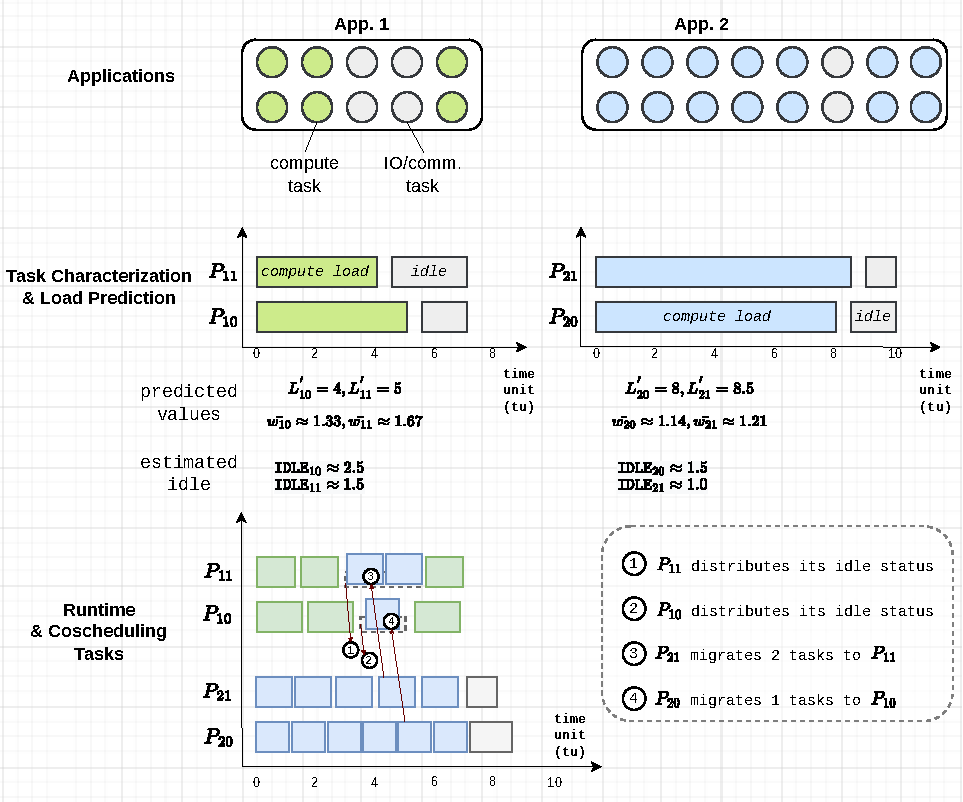
\includegraphics[scale=0.8]{./pictures/padlb_approach/padlb_coscheduling_idea_and_first_usecase.pdf}
	\caption{Co-scheduling strategy and the first use between two CPU applications.}
	\label{fig:proact_coschedule_task_and_first_usecase}
\end{figure}

Second, the procedure \texttt{proact\_coordinate\_TASK()} denotes how tasks are migrated to co-scheduling among the involved processes across different applications. There are two sides to the corresponding operations: one side of processes having idle slots and one side of processes being busy. At Line $9$, $10$, when an idle slot is detected, this information is distributed by the function \texttt{distribute()}. Otherwise, a process checks for receiving idle status from the others. If the idle status is received, a busy process can request offloading tasks (ranging from Line $11$ to $17$). Following that, the busy process waits for a confirmation to proceed with further task offloading if the number of expected tasks and idle slot is matched (indicated by Line $18$, $19$).\\

More intuitively, Figure \ref{fig:proact_coschedule_task_and_first_usecase} demonstrates the operations of Algorithm \ref{alg:proact_coschedule_task}. From top to bottom, we can loosely see three blocks denoted by \textbf{Applications}, \textbf{Task Characterization} \& \textbf{Load Prediction}, and \textbf{Runtime} \& \textbf{Coscheduling Tasks}. The scenario in this figure also illustrates the first use case of our co-scheduling method. In detail, each block is described as follows.

\begin{itemize}
	\item \textbf{Applications}: Two task-based applications are shown in the row of \textbf{Applications}, \texttt{App.1} and \texttt{App.2}. We assume that their tasks include compute tasks and IO/communication tasks. IO/communication tasks are considered idle slots because they are not compute-intensive but waiting for IO/communication. The CPU cores processing these tasks are idle for a period and can be switched to other compute tasks.
	\item \textbf{Task Characterization} \& \textbf{Load Prediction}: We address the stage of profiling tasks and predicting their load values. As illustrated, we give two processes per application; each process spawns multiple threads for executing tasks. Their IDs are indexed by the notation $P_{ij}$, where $i$ and $j$ indicate the index of application and process as mentioned above, e.g., $P_{10}$ indicates process $P_{0}$ belonging to application $1$. Suppose the prediction's results are ready; we have the predicted values of total load ($L^{'}_{ij}$), execution time per task ($w^{'}_{ij}$), and the idle time ($\texttt{IDLE}_{ij}$). For instance, application $1$ is shown with $L^{'}_{10}$, $L^{'}_{11}$, $w^{'}_{10}$, $w^{'}_{11}$, $\texttt{IDLE}_{10}$, and $\texttt{IDLE}_{11}$.
	\item \textbf{Runtime} \& \textbf{Coscheduling Tasks}: We show the illustrated events corresponding to the steps of procedure \texttt{proact\_coordinate\_TASK()} in Algorithm \ref{alg:proact_coschedule_task}. In this use case, \texttt{App.1} has idle slots, \texttt{App.2} is busier with more compute tasks. At the operations \circled{1}, \circled{2}, processes $P_{11}$ and $P_{10}$ of \texttt{App.1} distribute information about their idle status. In principle, after shaking-hand steps to reach an acceptance, process $P_{21}$ and $P_{20}$ of \texttt{App.2} migrates tasks to \texttt{App.1} to take advantage of the idle slots of \texttt{App.1} (shown as the operations \circled{3}, \circled{4}).
\end{itemize}

\begin{figure}[t]
	\centering
	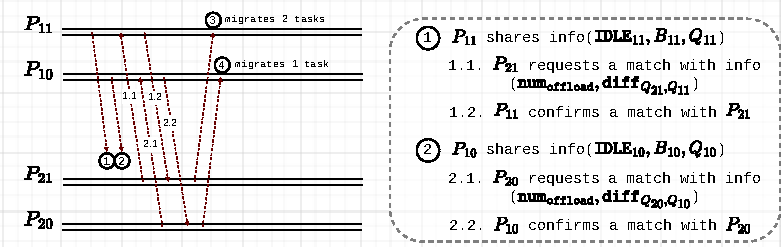
\includegraphics[scale=0.95]{./pictures/padlb_approach/padlb_coscheduling_protocol.pdf}
	\caption{A co-scheduling protocol for exchanging tasks with idle slots.}
	\label{fig:proact_coschedule_protocol}
\end{figure}

The operations \circled{1}, \circled{2}, \circled{3}, \circled{4} are detailed in Figure \ref{fig:proact_coschedule_protocol}. We have hand-shaking steps before tasks are offloaded. To ease the coordination between the processes of two applications, we distribute idle status associated with its estimated value, bandwidth information ($B$), and the current status of the queue. Bandwidth $B$ can be measured in advance and averaged gradually from the information exchange of previous steps. We attach it to calculate transmission time before offloading tasks. Furthermore, we need information about the current queue length to check how many remaining tasks there are and the queue lengths between the idle and busy processes. For example, $P_{11}$ distributes a message of $\texttt{IDLE}_{11}$, $B_{11}$, $Q_{11}$ at operation \circled{1}. On the side receiving idle status, the arrived information is checked first with the difference in queue length to ensure that there are still available tasks for migration. Then, we calculate a suitable number of tasks that should be offloaded from the busy process based on $\texttt{IDLE}$. The calculated amount of tasks should not exceed the capability of average bandwidth $B$ through a ratio, $\frac{\texttt{IDLE}\times B}{\texttt{data\_size}/task}$. Thereby, we can calculate how many tasks should fit the gap. For example, $P_{21}$ sends a request to match with $P_{11}$ at $1.1$ after calculating the number of available tasks. If $P_{11}$ agrees, it sends a confirmation message at $1.2$, and tasks are offloaded afterward. The selected victim for co-scheduling tasks during an idle period is ranked and prioritized from the sorted array of $\texttt{IDLE}^{'}$.\\

Several realistic HPC applications can represent the use case shown in Figure \ref{fig:proact_coschedule_task_and_first_usecase}. They have become more popular with large-scale simulations, such as environment issue simulations. More importantly, these applications must run with various scenarios and long-term tuning of the parameters for an optimal performance setup in HPC clusters. Hence, the idea of co-scheduling tasks in this method can be beneficial when one program has available idle slots, which are long enough to be replaced by tasks from another program. Our method can make both programs efficient and achieve better computing resource utilization. \\

For today's aspects with ML/DL applications, we illustrate another use case in Figure \ref{fig:proact_coschedule_second_usecase}. The x-axis shows time progress, while the y-axis highlights each application's processes and GPU region. The top is application $1$ (\texttt{App.1}), and the bottom is application 2 (\texttt{App.2}). Vertically, the process labels imply tasks executing on the CPU side (\texttt{CPU compute task}), while the GPU labels imply tasks executing on the GPU side (\texttt{GPU compute task}), and the blocks with dashed borders indicate idle slots. The main idea for applying our method to this use case includes:
\begin{itemize}
	\item An application has two types of tasks, \texttt{CPU compute task} and \texttt{GPU compute task}. Assuming when GPU tasks on an application are running, the CPU side is idle.
	\item When the CPU side of an application is idle, CPU tasks from another application can be migrated to fill the idle slots.
\end{itemize}

This use case becomes more familiar with heterogeneous architectures, i.e., CPU-GPU. In Figure \ref{fig:proact_coschedule_second_usecase}, we assume a distributed memory system of CPU-GPU nodes. We can share tasks during idle slots if tasks are well-defined.\\

% As illustrated in Figure \ref{fig:proact_coschedule_second_usecase}, there are also two applications, but tasks include CPU-GPU tasks and idle slots for waiting data movement between both sides.  Similarly, tasks from the busy side are migrated to the idle side with an estimation of communication overhead. \\

\begin{figure}[t]
	\centering
	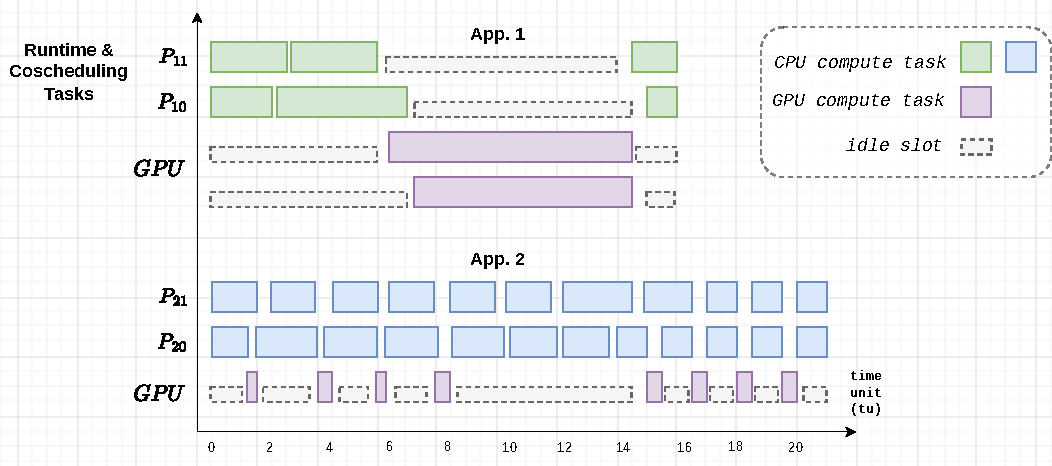
\includegraphics[scale=0.85]{./pictures/padlb_approach/padlb_coscheduling_second_usecase.pdf}
	\caption{The second use case of proactive coscheduling tasks.}
	\label{fig:proact_coschedule_second_usecase}
\end{figure}

In the following chapters, we will show the implementation of our two methods and this extension. Significantly, with this extension for co-scheduling tasks, we cannot interfere with the execution of jobs in HPC clusters due to permission. Therefore, the experiments are emulated by defining different tasks in an executable, representing multiple applications that run simultaneously. Different tasks from different applications are in the same executable. For example, there is a whole job executing on $4$ compute nodes, where two nodes will host the first application with its tasks, and the remaining nodes will host the second application. In such a submitted job, the two applications run simultaneously, enabling MPI to provide the same communication environment between them.

% One advantage of task-based applications is an abstraction of task definition, which points to the code and data. Therefore, it is feasible to profile the characteristics of tasks, e.g., inputs, outputs, that we can combine with system information, e.g., core frequencies, performance counters, to predict the load values. 




% While the load balance is expected before running the applications, another challenge could be caused at the system side when some machines/processes can slow down. The unexpected situation needs actions at runtime and faces the challenge of moving tasks around to regain the balance as expected. Suppose there is no prior knowledge to redistribute the tasks. In that case, people have to use work-stealing ideas in principle, and the delay of stealing time on distributed memory is the challenge. Therefore, the approach in this thesis could be described in the inline figure below.\\

% What we can have is usually queue length status and execution speed. The balancing strategies have to decide which tasks are migrated, from which rank to which rank. We know little about the execution speed based on the number of remaining tasks in queues per rank or even per machine. All in all, the outcome of almost balancing solutions resolves around:

%In general, we introduce one proactive approach, which can provide different load-balancing strategies at runtime. The more information we have at runtime, the better strategies we can perform for dynamic load balancing.

%\begin{enumerate}
%	\item Which process shares tasks to which process?
%	\item And, how many tasks should be migrated at a time?
%\end{enumerate}

% We then use the prediction to provide the missing knowledge about load at runtime and guide task offloading. Therefore, as mentioned above, we have partial load information to calculate well (1) and (2). Additionally, we can generate different strategies for task offloading.\\

%From the runtime point of view, we can see that our programs are performed with multiple processes or MPI ranks in distributed memory. In which each process spawns multiple threads to execute tasks, and each thread is pinned to one core. Notably, one dedicated thread is pinned to the last core to perform proactive load balancing. For modern computing architectures today, we have many sockets (even GPU as accelerators) in a single machine; a socket has many cores for parallel processing. At the operating system level, one process can spawn as many threads as recommended to fit the maximum number of physical cores per socket.